% Created by tikzDevice version 0.6.2-92-0ad2792 on 2012-11-14 12:23:54
% !TEX encoding = UTF-8 Unicode
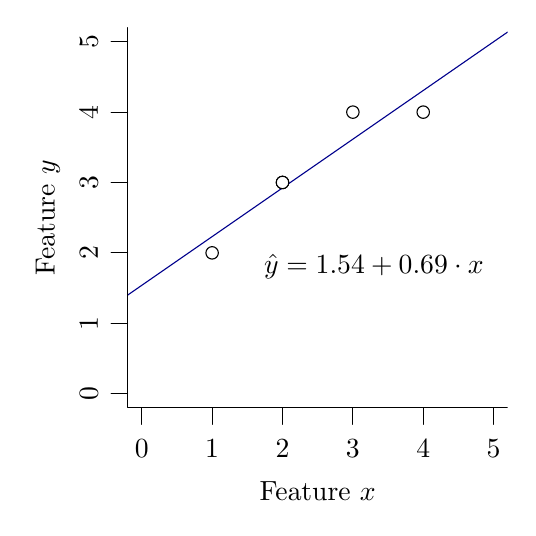
\begin{tikzpicture}[x=1pt,y=1pt]
\definecolor[named]{fillColor}{rgb}{1.00,1.00,1.00}
\path[use as bounding box,fill=fillColor,fill opacity=0.00] (0,0) rectangle (173.45,173.45);
\begin{scope}
\path[clip] (  0.00,  0.00) rectangle (173.45,173.45);
\definecolor[named]{drawColor}{rgb}{0.00,0.00,0.00}

\node[text=drawColor,anchor=base,inner sep=0pt, outer sep=0pt, scale=
  1.00] at (104.79,  2.54) {Feature $x$};

\node[text=drawColor,rotate= 90.00,anchor=base,inner sep=0pt, outer
  sep=0pt, scale=  1.00] at (  9.73,104.79) {Feature $y$};
\end{scope}
\begin{scope}
\path[clip] ( 36.13, 36.13) rectangle (173.45,173.45);
\definecolor[named]{drawColor}{rgb}{0.00,0.00,0.55}

\path[draw=drawColor,line width= 0.4pt,line join=round,line cap=round] ( 36.13, 76.82) -- (173.45,171.88);
\definecolor[named]{drawColor}{rgb}{0.00,0.00,0.00}
\definecolor[named]{fillColor}{rgb}{1.00,1.00,1.00}

\path[draw=drawColor,line width= 0.4pt,line join=round,line cap=round,fill=fillColor] ( 92.08,117.51) circle (  2.25);

\path[draw=drawColor,line width= 0.4pt,line join=round,line cap=round,fill=fillColor] ( 66.65, 92.08) circle (  2.25);

\path[draw=drawColor,line width= 0.4pt,line join=round,line cap=round,fill=fillColor] (117.51,142.93) circle (  2.25);

\path[draw=drawColor,line width= 0.4pt,line join=round,line cap=round,fill=fillColor] ( 92.08,117.51) circle (  2.25);

\path[draw=drawColor,line width= 0.4pt,line join=round,line cap=round,fill=fillColor] (142.93,142.93) circle (  2.25);

\node[text=drawColor,anchor=base,inner sep=0pt, outer sep=0pt, scale=  1.00] at (125.13, 84.49) {$\hat{y} = 1.54 + 0.69 \cdot x$};
\end{scope}
\begin{scope}
\path[clip] (  0.00,  0.00) rectangle (173.45,173.45);
\definecolor[named]{drawColor}{rgb}{0.00,0.00,0.00}

\path[draw=drawColor,line width= 0.4pt,line join=round,line cap=round] ( 41.22, 36.13) -- (168.36, 36.13);

\path[draw=drawColor,line width= 0.4pt,line join=round,line cap=round] ( 41.22, 36.13) -- ( 41.22, 30.13);

\path[draw=drawColor,line width= 0.4pt,line join=round,line cap=round] ( 66.65, 36.13) -- ( 66.65, 30.13);

\path[draw=drawColor,line width= 0.4pt,line join=round,line cap=round] ( 92.08, 36.13) -- ( 92.08, 30.13);

\path[draw=drawColor,line width= 0.4pt,line join=round,line cap=round] (117.51, 36.13) -- (117.51, 30.13);

\path[draw=drawColor,line width= 0.4pt,line join=round,line cap=round] (142.93, 36.13) -- (142.93, 30.13);

\path[draw=drawColor,line width= 0.4pt,line join=round,line cap=round] (168.36, 36.13) -- (168.36, 30.13);

\node[text=drawColor,anchor=base,inner sep=0pt, outer sep=0pt, scale=  1.00] at ( 41.22, 18.13) {0};

\node[text=drawColor,anchor=base,inner sep=0pt, outer sep=0pt, scale=  1.00] at ( 66.65, 18.13) {1};

\node[text=drawColor,anchor=base,inner sep=0pt, outer sep=0pt, scale=  1.00] at ( 92.08, 18.13) {2};

\node[text=drawColor,anchor=base,inner sep=0pt, outer sep=0pt, scale=  1.00] at (117.51, 18.13) {3};

\node[text=drawColor,anchor=base,inner sep=0pt, outer sep=0pt, scale=  1.00] at (142.93, 18.13) {4};

\node[text=drawColor,anchor=base,inner sep=0pt, outer sep=0pt, scale=  1.00] at (168.36, 18.13) {5};

\path[draw=drawColor,line width= 0.4pt,line join=round,line cap=round] ( 36.13, 41.22) -- ( 36.13,168.36);

\path[draw=drawColor,line width= 0.4pt,line join=round,line cap=round] ( 36.13, 41.22) -- ( 30.13, 41.22);

\path[draw=drawColor,line width= 0.4pt,line join=round,line cap=round] ( 36.13, 66.65) -- ( 30.13, 66.65);

\path[draw=drawColor,line width= 0.4pt,line join=round,line cap=round] ( 36.13, 92.08) -- ( 30.13, 92.08);

\path[draw=drawColor,line width= 0.4pt,line join=round,line cap=round] ( 36.13,117.51) -- ( 30.13,117.51);

\path[draw=drawColor,line width= 0.4pt,line join=round,line cap=round] ( 36.13,142.93) -- ( 30.13,142.93);

\path[draw=drawColor,line width= 0.4pt,line join=round,line cap=round] ( 36.13,168.36) -- ( 30.13,168.36);

\node[text=drawColor,rotate= 90.00,anchor=base,inner sep=0pt, outer sep=0pt, scale=  1.00] at ( 25.33, 41.22) {0};

\node[text=drawColor,rotate= 90.00,anchor=base,inner sep=0pt, outer sep=0pt, scale=  1.00] at ( 25.33, 66.65) {1};

\node[text=drawColor,rotate= 90.00,anchor=base,inner sep=0pt, outer sep=0pt, scale=  1.00] at ( 25.33, 92.08) {2};

\node[text=drawColor,rotate= 90.00,anchor=base,inner sep=0pt, outer sep=0pt, scale=  1.00] at ( 25.33,117.51) {3};

\node[text=drawColor,rotate= 90.00,anchor=base,inner sep=0pt, outer sep=0pt, scale=  1.00] at ( 25.33,142.93) {4};

\node[text=drawColor,rotate= 90.00,anchor=base,inner sep=0pt, outer sep=0pt, scale=  1.00] at ( 25.33,168.36) {5};

\path[draw=drawColor,line width= 0.4pt,line join=round,line cap=round] ( 36.13,173.45) --
	( 36.13, 36.13) --
	(173.45, 36.13);
\end{scope}
\end{tikzpicture}
